\documentclass{article}
\usepackage[utf8]{inputenc}
%\usepackage[english]{babel}
\usepackage[portuguese]{babel}
\usepackage{graphicx}
\usepackage[hidelinks]{hyperref}
\usepackage{amsmath} %lets us use \begin{proof}
%\usepackage[]{amssymb} %gives us the character \varnothing
\usepackage[dvipsnames]{xcolor}
\usepackage{verbatim}

\title{Universidade Federal de Pernambuco \\
Macroeconomia 2 - Lista 1}
\author{Monitor: Paulo Silva}
\date{11 de novembro de 2022}

\begin{document}
\maketitle %This command prints the title based on information entered above

%Section and subsection automatically number unless you put the asterisk next to them.

\section*{Questão 2}
Sabemos que: $$U = \ln(C_c) + \beta \ln(C_1); \>\>\> 
Y_0 = 100; \>\>\>
Y_1 = 50; \>\>\>
r = 0; \>\>\>
\beta = 1; $$
Podemos derivar a restrição orçamentária intertemporal como:

\begin{equation}\label{eq:2roi}
    C_0 + \frac{C_1}{(1+r)} = Y_0 + \frac{ Y_1}{(1+r)};
\end{equation}
\\
Queremos $\max_{n} U(C_0,C_1)$ s.a R.O.I \eqref{eq:2roi}:

\begin{equation}
    L = \ln(C_0)+\beta\ln(C_1)-\lambda\left[ C_0+\frac{C_1}{(1+r)}-Y_0-\frac{Y_1}{(1+r)}  \right]
\end{equation}
\\
Logo, as C.P.O são dadas por:
\begin{equation}\label{eq:2cporoc0}
    \frac{\partial L}{\partial C_0} = \frac{1}{C_0} - \lambda=0 \to \lambda = \frac{1}{C_0}
\end{equation}

\begin{equation}\label{eq:2cporoc1}
    \frac{\partial L}{\partial C_1} = \frac{\beta}{C_1}-\frac{\lambda}{(1+r)}=0 \to \lambda = \frac{(1+r)\beta}{C_1}
\end{equation}
\\
Igualando os lambdas das equações \eqref{eq:2cporoc0} e \eqref{eq:2cporoc1} e aplicando $r=0$, $\beta=1$, temos:
\begin{equation}\label{eq:2eqlambda}
    \frac{1}{C_0} = \frac{(1+r)\beta}{C_1}
\end{equation}

\begin{equation}
    \frac{1}{C_0} = \frac{1}{C_1} \to C_0^* = C_1^*
\end{equation}
\\
Aplicando os dados do enunciado e da equação \eqref{eq:2eqlambda} na R.O.I:
\begin{equation}
    C_0 + C_0 = Y_0 + Y_1
\end{equation}

\begin{equation}
    2C_0 = Y_0 + Y_1
\end{equation}

\begin{equation}
    C_0 = \frac{Y_0 + Y_1}{2}
\end{equation}

\begin{equation}
    C_0^* = C_1^* = \frac{150}{2} = 75
\end{equation}
\\
Como $C_0 = C_1$ dado por \eqref{eq:2eqlambda}, o consumo por período será igual a 75 unidades.
\\ \\
A poupança é determinada através de $C_0^* + S_0 = Y_0$, assim, temos:
\begin{equation}
    S_0 = Y_0 - C_0^*
\end{equation}

\begin{equation}
    S_0 = 100 - 75 = 25
\end{equation}

Graficamente, temos:
\begin{figure}[!tbh]
    \centering
    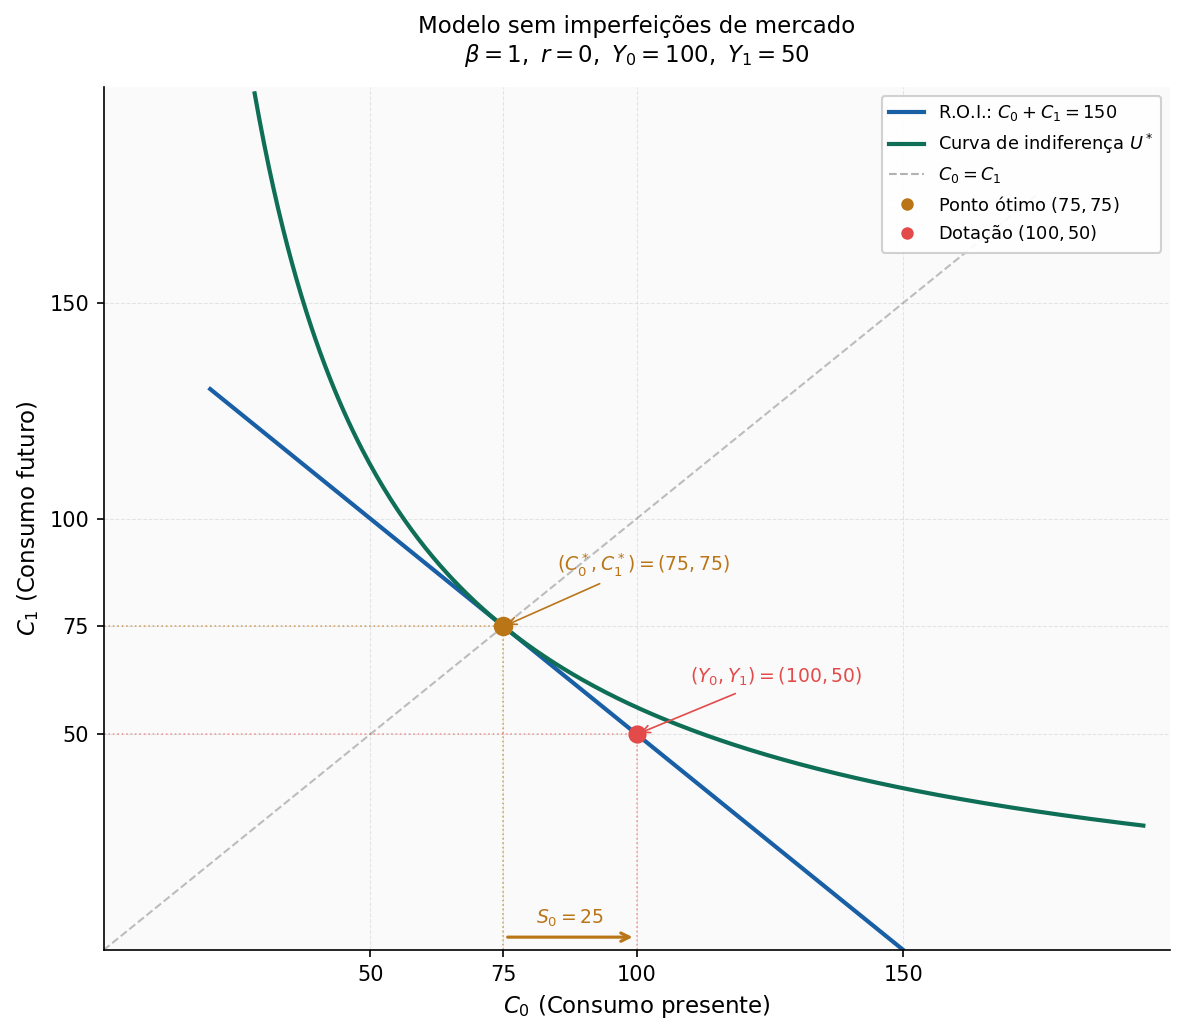
\includegraphics[width=\textwidth]{Q2.png}
    \caption{Modelo sem imperfeições de mercado}
    \label{fig:GMC1}
\end{figure}

\clearpage

\section*{Questão 3}
Do enunciado, temos:
$$U=c_{1}^{\alpha}c_{2}^{1-\alpha}; \>\>\> 
r=0.2; \>\>\> 
Y_1=80; \>\>\>
Y_2=100; \>\>\>
\alpha=0.5 $$
\\
Podemos derivar a restrição orçamentária intertemporal como:
\begin{equation}\label{eq:3roi}
    c_1 + \frac{c_2}{(1+r)} = Y_1 + \frac{Y_2}{(1+r)};
\end{equation}
\\
Podemos linearizar a função utilidade conforme:
\begin{equation}
    \ln U = \alpha\ln c_1+(1-\alpha)\ln c_2
\end{equation}
\\
Queremos $\max_{n} U(c_1,c_2)$ s.a R.O.I \eqref{eq:3roi}:

\begin{equation}
    L = \alpha\ln c_1+(1-\alpha)\ln c_2-\lambda\left[ c_1+\frac{c_2}{(1+r)}-Y_1-\frac{Y_2}{(1+r)}  \right]
\end{equation}
\\
Logo, as C.P.O são dadas por:
\begin{equation}\label{eq:3cpoc1}
    \frac{\partial L}{\partial c_1} = \frac{\alpha}{c_1}-\lambda=0 \to \lambda = \frac{\alpha}{c_1}
\end{equation}

\begin{equation}\label{eq:3cpoc2}
    \frac{\partial L}{\partial c_2} = \frac{(1-\alpha)}{c_2}-\frac{\lambda}{(1+r)}=0 \to \lambda = \frac{(1-\alpha)(1+r)}{c_2}
\end{equation}
\\
Igualando os lambdas, e substituindo valores temos:
\begin{equation}
    \frac{\alpha}{c_1} = \frac{(1-\alpha)(1+r)}{c_2}
\end{equation}
\begin{equation}
    c_2 = \frac{(1-\alpha)(1+r)c_1}{\alpha}
\end{equation}
\begin{equation}
    c_2 = \frac{(0.5)(1,2)c_1}{0.5} \to c_2^* = 1,2 c_1^*
\end{equation}
\begin{equation}\label{eq:3eqlambda}
    c_2^* = 1,2 c_1^*
\end{equation}
\\
Substituindo então \eqref{eq:3eqlambda} na R.O.I \eqref{eq:3roi}, com valores:
\begin{equation}
     c_1 + \frac{1,2c_1}{1,2} = 80 + \frac{100}{(1,2)} \to 2c_1 = 163,333333 \to c_1 \approx 81,666666
\end{equation}

\begin{equation}
    c_2 = 1,2c_1 \to c_2 = 1,2*81,666666 \to c_2 \approx 97,999999
\end{equation}
\\
O consumo em $c_1$ e $c_2$ será respectivamente 81,666666 e 97,999999.

\clearpage
\clearpage
\section*{Questão 4}
\subsection*{Letra i)}
A queda da renda das famílias no primeiro período leva a uma queda na dotação e, portanto, da riqueza intertemporal, deslocando a ROI paralelamente para baixo(dentro), dada que a taxa de juros é a mesma. Como ambos os bens são normais, buscando suavizar o consumo, a família distribui a queda na renda nos dois períodos. A queda no consumo em $t=1$ é menor que a queda na renda em $t=1$ $\implies$ a poupança fica mais negativa. O consumo do período dois também cai. Um novo ponto ótimo é tal que $C_1$ e $C_2$ são menores. 
\begin{figure}[!tbh]
    \centering
    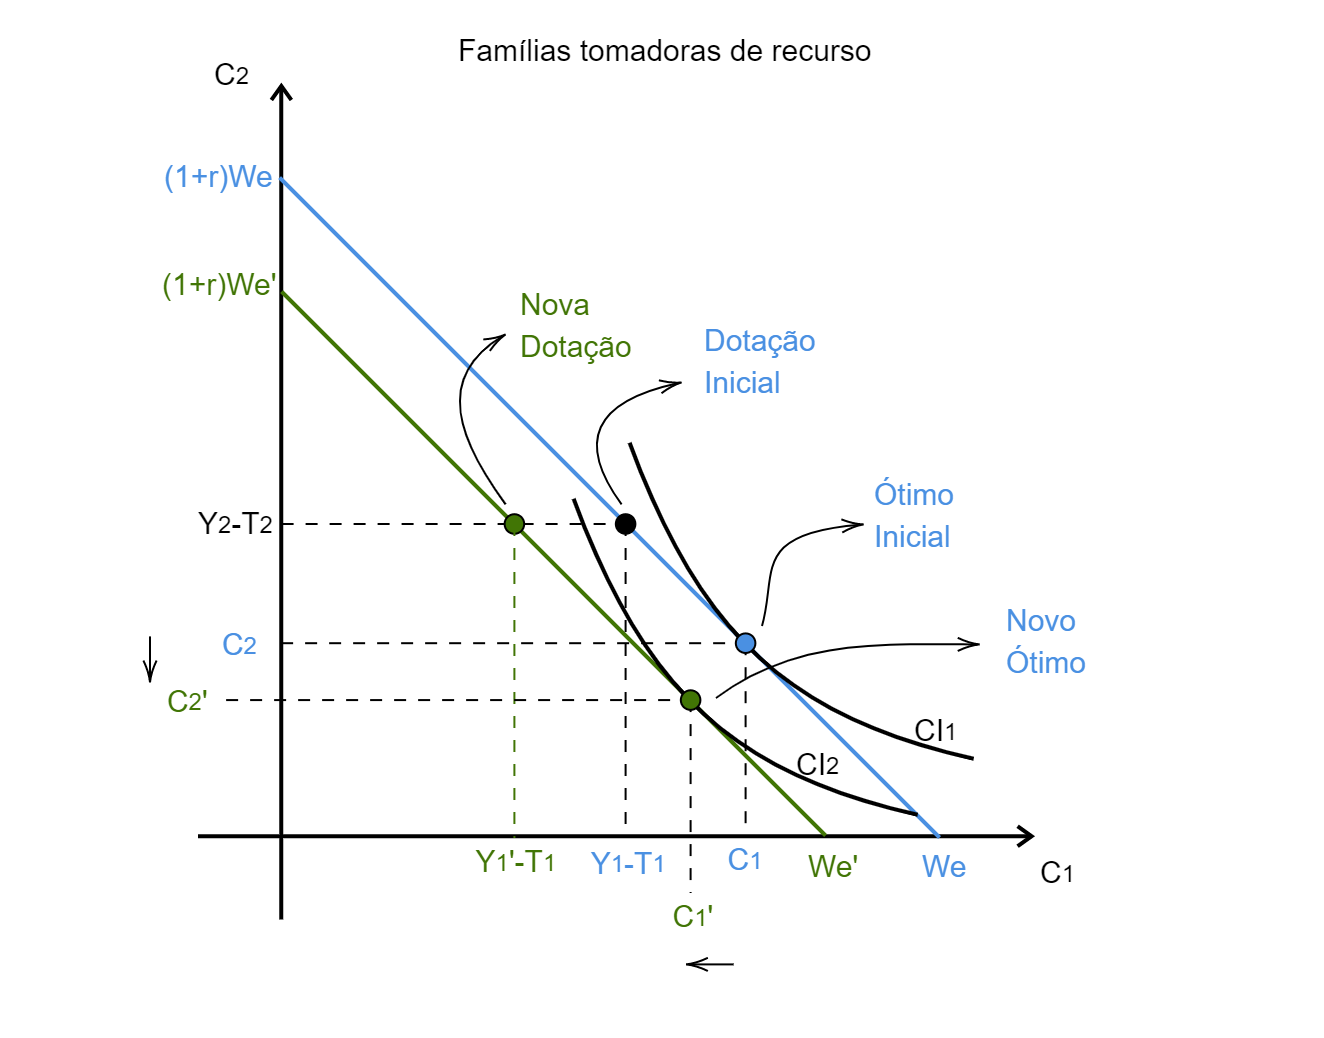
\includegraphics[width=\textwidth]{Q41.png}
    \caption{Queda na renda em t=1 para família tomadora}
\end{figure}
\clearpage
\subsection*{Letra ii)}
A queda da renda das famílias no primeiro período leva a uma queda na dotação e, portanto, da riqueza intertemporal, deslocando a ROI paralelamente para baixo(dentro), dada que a taxa de juros é a mesma. Como ambos os bens são normais, buscando suavizar o consumo, a família distribui a queda na renda nos dois períodos. A queda no consumo em $t=1$ é menor que a queda na renda em $t=1$ $\implies$ a poupança fica menor. O consumo do período dois também cai. Um novo ponto ótimo é tal que $C_1$ e $C_2$ são menores. 
\begin{figure}[!tbh]
    \centering
    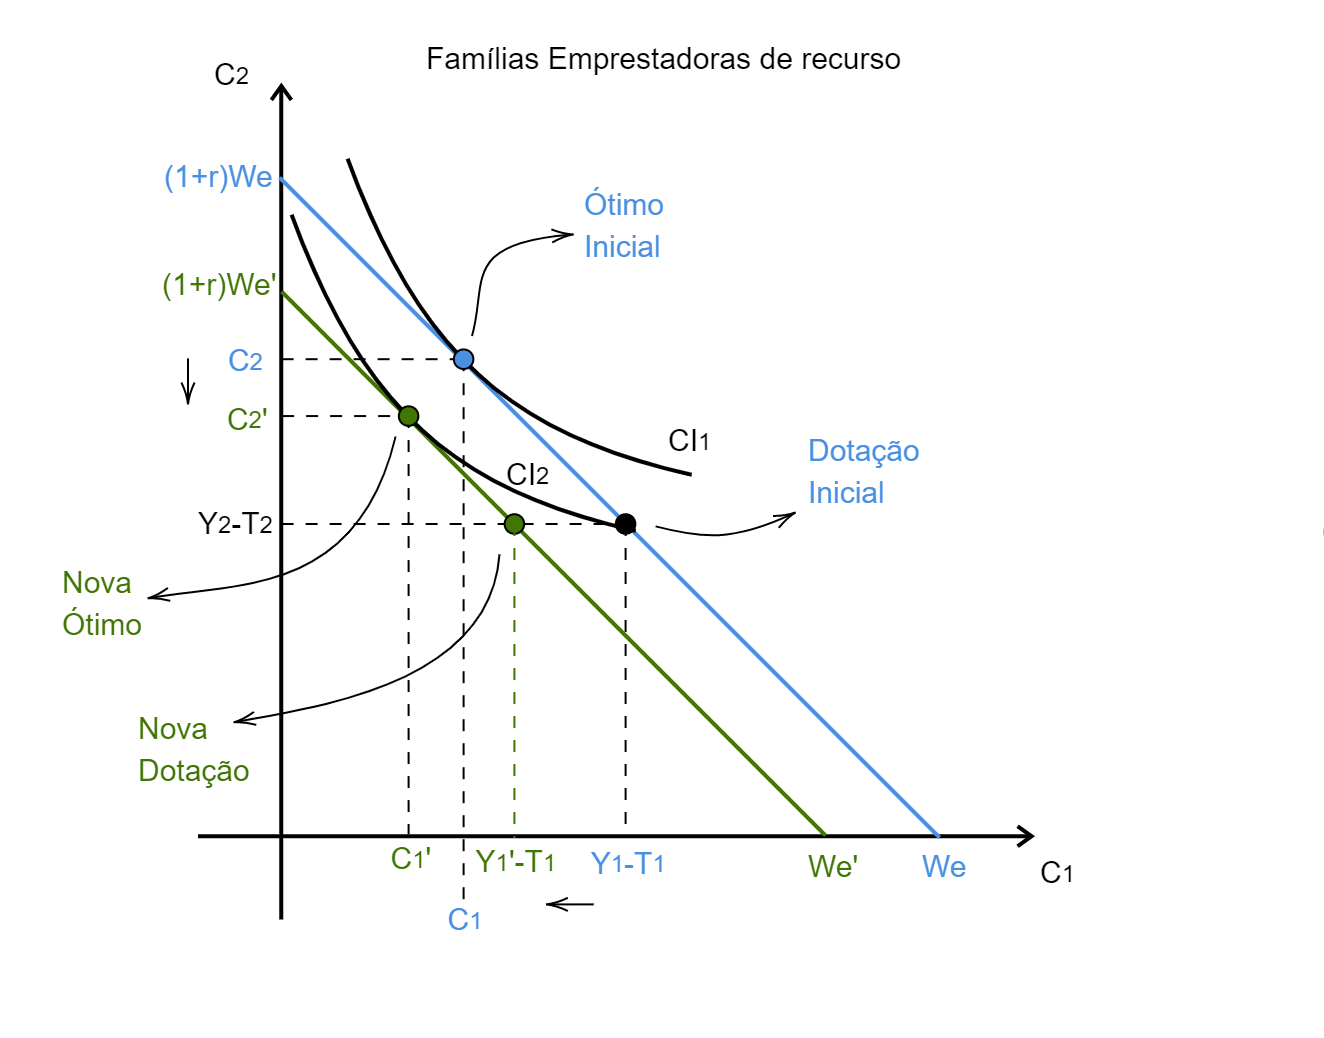
\includegraphics[width=\textwidth]{Q42.png}
    \caption{Queda na renda em t=1 para família tomadora}
\end{figure}

\clearpage
\section*{Questão 6}
Podemos derivar a restrição orçamentária como:
\begin{equation}\label{eq:6roi}
    C_1 + \frac{C_2}{(1+r)} = Y_1 - T_1 + \frac{Y_2-T_2}{(1+r)}
\end{equation}

\subsection*{Letra A)}
Dado o enunciado têm-se: 
$$\beta = 1; \>\>\> Y_1=1000; \>\>\> Y_2=1200; \>\>\> T_1=200; \>\>\> T_2=100; \>\>\> r=0.1;$$
Montando o lagrangiano e realizando C.P.O:
\begin{equation}
    L = \ln C_1 + \beta\ln C_2 - \lambda\left[C_1+\frac{C_2}{(1+r)}-Y_1+T_1-\frac{Y_2-T_2}{(1+r)}\right]
\end{equation}

\begin{equation}\label{eq:6cpoc1}
    \frac{\partial L}{\partial C_1} = \frac{1}{C_1} - \lambda = 0 \to \lambda=\frac{1}{C_1}
\end{equation}

\begin{equation}\label{eq:6cpoc2}
    \frac{\partial L}{\partial C_2} = \frac{\beta}{C_2} - \frac{\lambda}{(1+r)} = 0 \to \lambda = \frac{(1+r)\beta}{C_2}
\end{equation}
\\
Igualando os lambdas das equações \eqref{eq:6cpoc1} e \eqref{eq:6cpoc2}, e substituindo $\beta=1$:
\begin{equation}\label{eq:6eqlambda}
    C_1=\frac{C_2}{(1+r)} \>\>\> ou \>\>\> C_2=C_1(1+r)
\end{equation}
\\
Substituindo \eqref{eq:6eqlambda} em \eqref{eq:6roi}, têm-se o consumo ótimo do primeiro período:
\begin{equation}
    C_1 + \frac{C_1(1+r)}{(1+r)} = Y_1 - T_1 + \frac{Y_2-T_2}{(1+r)}
\end{equation}

\begin{equation}
    2C_1 = Y_1 - T_1 + \frac{Y_2-T_2}{(1+r)}
\end{equation}

\begin{equation}
    C_1^* = \left[Y_1 - T_1 + \frac{Y_2-T_2}{(1+r)}\right]\frac{1}{2}
\end{equation}
\\
Substituindo valores, encontramos as quantidades ótimas:
\begin{equation}
    C_1^* = \left[1000 - 200 + \frac{1200-100}{(1,1)}\right]\frac{1}{2} \to C_1^* = \frac{1800}{2} = 900
\end{equation}

\begin{equation}
    C_2^* = (1+r)C_1^* \to C_2^* = 1,1*900 = 990
\end{equation}

\begin{equation}
    S_1^* = Y_1-T_1-C_1^* \to S_1^*=1000-200-900 = -100
\end{equation}
\clearpage

\subsection*{Letra B)}
Podemos derivar a R.O.G como:
\begin{equation}\label{eq:6Brog}
    G_1 + \frac{G_2}{(1+r)} = T_1 + \frac{T_2}{(1+r)}
\end{equation}
\\
Sabemos que $G_1=G_2=T_1=T_2=\bar{T}$, e ainda $T_{1}^{'}=T_1-\delta$, portanto, teremos:
\begin{equation}\label{eq:6bt1}
    T_{1}^{'}=\bar{T}-\delta
\end{equation}
\begin{equation}
    \bar{T}+\frac{\bar{T}}{(1+r)}=\bar{T}-\delta+\frac{T_2}{(1+r)}
\end{equation}
\\
Isolando $T_2$, encontramos o aumento que deve ser promovido no segundo período:
\begin{equation}\label{eq:6bt2}
    T_2=\bar{T}+\delta(1+r)
\end{equation}
\\
A R.O.I das famílias é dada por:
\begin{equation}\label{eq:6Broi}
    C_1 + \frac{C_2}{(1+r)} = Y_1 - T_1 + \frac{Y_2}{(1+r)}-\frac{T_2}{(1+r)}
\end{equation}
\\
Substituindo então as alterações de impostos \eqref{eq:6bt1} e \eqref{eq:6bt2} na R.O.I \eqref{eq:6Broi}:
\begin{equation}
    C_1 + \frac{C_2}{(1+r)} = Y_1 - \bar{T}+\delta + \frac{Y_2}{(1+r)}-\frac{\bar{T}+\delta(1+r)}{(1+r)}
\end{equation}

\begin{equation}
    C_1 + \frac{C_2}{(1+r)} = Y_1 - \bar{T}+\delta + \frac{Y_2}{(1+r)}-\frac{\bar{T}}{(1+r)}-\delta
\end{equation}

\begin{equation}
    C_1 + \frac{C_2}{(1+r)} = Y_1 - \bar{T}+ + \frac{Y_2}{(1+r)}-\frac{\bar{T}}{(1+r)}
\end{equation}
\\
Note que $\bar{T}=T_1=T_2$, logo a R.O.I é a mesma, não alterou a riqueza ou escolhas ótimas das famílias, e portanto a equivalência Ricardiana é observada.
\clearpage
\section*{Questão 8}
Sabemos que:
$$C_1 + S_1 = Y_1; \>\>\> C_2 = Y_2 + (1+r)S_1; \>\>\> Y_2 = (1-\theta)Y_1$$
Organizando as três equações, encontramos a R.O.I:
\begin{equation}\label{eq:8Aroi}
    C_1+\frac{C_2}{(1+r)}=Y_1+\frac{(1-\theta)Y_1}{(1+r)}
\end{equation}

\subsection*{Letra A)}
Montando o lagrangiano e otimizando, temos as seguintes C.P.O:
\begin{equation}
    L=\ln C_1 + \beta\ln C_2-\lambda\left[C_1+\frac{C_2}{(1+r)}-Y_1-\frac{(1-\theta)Y_1}{(1+r)}\right]
\end{equation}

\begin{equation}
    \frac{\partial L}{\partial C_1} = \frac{1}{C_1} -\lambda=0 \to \lambda=\frac{1}{C_1}
\end{equation}

\begin{equation}
    \frac{\partial L}{\partial C_2}=\frac{\beta}{C_2}-\frac{\lambda}{(1+r)} =0 \to \lambda=\frac{\beta(1+r)}{C_2}
\end{equation}
\\
Igualando os lambdas, temos:
\begin{equation}\label{eq:8Aeqlambda}
    C_1=\frac{C_2}{\beta(1+r)} \>\>\> ou \>\>\> C_2=C_1\beta(1+r)
\end{equation}
\\
Substituindo o resultado anterior \eqref{eq:8Aeqlambda} na R.O.I \eqref{eq:8Aroi}, e isolando $C_1$:
\begin{equation}
    C_1+\frac{C_1\beta(1+r)}{(1+r)} = Y_1 + \frac{(1-\theta)Y_1}{(1+r)}
\end{equation}

\begin{equation}
    (1+\beta)C_1 = Y_1 + \frac{(1-\theta)Y_1}{(1+r)}
\end{equation}
\\
O consumo ótimo no período 1 é dado por:
\begin{equation}\label{eq:8ac1star}
    C_1^* = \frac{Y_1}{(1+\beta)} + \frac{(1-\theta)Y_1}{(1+r)(1+\beta)}
\end{equation}
\\
Substituindo \eqref{eq:8ac1star} em \eqref{eq:8Aeqlambda}, encontramos o consumo ótimo em t=2:
\begin{equation}
    C_2^*=\beta(1+r)\left[\frac{Y_1}{(1+\beta)} + \frac{(1-\theta)Y_1}{(1+r)(1+\beta)}\right]
\end{equation}

\begin{equation}
    C_2^*=\frac{\beta(1+r)Y_1}{(1+\beta)} + \beta\frac{(1-\theta)Y_1}{(1+\beta)}
\end{equation}
\\
Podemos encontrar a poupança ótima fazendo:
\begin{equation}
    S_1^* = Y_1 - C_1^*
\end{equation}

\begin{equation}
    S_1^* = Y_1 - \frac{Y_1}{(1+\beta)} - \frac{(1-\theta)Y_1}{(1+r)(1+\beta)}
\end{equation}
\\
Os efeitos de um aumento em teta são dados por:
\begin{equation}
    \frac{\partial C_1}{\partial \theta} = -\frac{Y_1}{(1+r)(1+\beta)} <0     
\end{equation}

\begin{equation}
    \frac{\partial C_2}{\partial \theta} = -\beta\frac{Y_1}{(1+\beta)} <0     
\end{equation}

\begin{equation}
    \frac{\partial S_1}{\partial \theta} = \frac{Y_1}{(1+r)(1+\beta)} >0     
\end{equation}
\\
$\theta$ governa o quanto a renda do segundo período será menor que a renda do primeiro. No caso limite, quando $\theta = 0$, a renda seria a mesma e se $\theta=1$, a renda do segundo período seria zero. Então quanto maior for esse parâmetro, menor será a renda do segundo período. Portanto, quando $\theta \uparrow \implies$ uma queda na renda do segundo período, o que faz a família reduzir consumo nos dois períodos. A família otimamente antecipa que ficará mais pobre e, portanto, precisa transferir mais renda do primeiro para o segundo período, compensando parcialmente a queda na renda futura. Com isso a poupança sobe com a queda na renda futura. 

\subsection*{Letra B)}
Podemos reescrever a R.O.I como:
\begin{equation}\label{eq:8Broi}
    (1+\tau_1)C_1+\frac{(1+\tau_2)C_2}{(1+r)}=Y_1+\frac{(1-\theta)Y_1}{(1+r)}
\end{equation}
\\
Assim, maximizando a utilidade s.a R.O.I:
\begin{equation}
    L=\ln C_1 + \beta\ln C_2-\lambda\left[(1+\tau_1)C_1+\frac{(1+\tau_2)C_2}{(1+r)}-Y_1-\frac{(1-\theta)Y_1}{(1+r)}\right]
\end{equation}

\begin{equation}
    \frac{\partial L}{\partial C_1}=\frac{1}{C_1}-(1+\tau_1) \lambda=0 \to \lambda=\frac{1}{(1+\tau_1)C_1}
\end{equation}

\begin{equation}
    \frac{\partial L}{\partial C_2}=\frac{\beta}{C_2}-\lambda\frac{(1+\tau_2)}{(1+r)}=0 \to \lambda = \frac{\beta(1+r)}{C_2(1+\tau_2)}
\end{equation}
\\
Igualando os lambdas temos:
\begin{equation}
    \frac{1}{(1+\tau_1)C_1}=\frac{\beta(1+r)}{C_2(1+\tau_2)}
\end{equation}

\begin{equation}\label{eq:8Beqlambda}
    C_2=\frac{\beta(1+r)(1+\tau_1)C_1}{(1+\tau_2)}
\end{equation}
\\
Substituindo \eqref{eq:8Beqlambda} na nova R.O.I:
\begin{equation}
    (1+\tau_1)C_1+\frac{(1+\tau_2)}{(1+r)}\frac{\beta(1+r)(1+\tau_1)C_1}{(1+\tau_2)}=Y_1+\frac{(1-\theta)Y_1}{(1+r)}
\end{equation}

\begin{equation}
    (1+\tau_1)C_1+\beta(1+\tau_1)C_1=Y_1+\frac{(1-\theta)Y_1}{(1+r)}
\end{equation}

\begin{equation}
    (1+\tau_1)(1+\beta)C_1=Y_1+\frac{(1-\theta)Y_1}{(1+r)}
\end{equation}

\begin{equation}\label{eq:8bc1star}
    C_1^*=\left[ Y_1+\frac{(1-\theta)Y_1}{(1+r)}\right]\frac{1}{(1+\tau_1)(1+\beta)}
\end{equation}
\\
Substituindo $C_1^*$ \eqref{eq:8bc1star} em $C_2$, temos:
\begin{equation}
    C_2=\frac{\beta(1+r)(1+\tau_1)}{(1+\tau_2)}\left[ Y_1+\frac{(1-\theta)Y_1}{(1+r)}\right]\frac{1}{(1+\tau_1)(1+\beta)}
\end{equation}

\begin{equation}
    C_2^*=\frac{\beta(1+r)}{(1+\tau_2)(1+\beta)}\left[ Y_1+\frac{(1-\theta)Y_1}{(1+r)}\right]
\end{equation}
\\
A poupança é derivada da nova R.O em t=1, $S_1^*=Y_1- (1+\tau_1)C_1^*$ , portanto:
\begin{equation}
    S_1^*=Y_1-(1+\tau_1)\left[ Y_1+\frac{(1-\theta)Y_1}{(1+r)}\right]\frac{1}{(1+\tau_1)(1+\beta)}
\end{equation}
\begin{equation}
    S_1^*=Y_1-\left[ Y_1+\frac{(1-\theta)Y_1}{(1+r)}\right]\frac{1}{(1+\beta)}
\end{equation}
\\
Ou seja, os efeitos de um aumento em $\tau_1$ são:

\begin{equation}
    \frac{\partial C_1^*}{\partial\tau_1}=-\left[ Y_1+\frac{(1-\theta)Y_1}{(1+r)}\right]\frac{1}{(1+\tau_1)^2(1+\beta)} < 0
\end{equation}

\begin{equation}
    \frac{\partial S_1^*}{\partial\tau_1} = 0
\end{equation}

\begin{equation}
    \frac{\partial C_2^*}{\partial\tau_1} = 0 
\end{equation}
\\
Um aumento em $\tau_1$ reduz a escolha ótima de consumo das famílias no período um. Nem a poupança, nem o consumo em t=2 respondem. O recurso extra salvo pela queda consumo em t=1 é usado para pagar o imposto mais alto.
\clearpage

\section*{Questão 11}
Dados fornecido pelo enunciado:
$$U=\log(C_1)+\beta\log(C_2);\>\>\>
\beta=0.5\>\>\> r=0.05$$
Montando o lagrangiano e maximizando, temos:
\begin{equation}
    L=\log(C_1)+\beta\log(C_2)-\lambda\left[C_1+\frac{C_2}{(1+r)}-Y_1-\frac{Y_2}{(1+r)}\right]
\end{equation}
\begin{equation}\label{eq:11c1}
    \frac{\partial L}{\partial C_1}=\frac{1}{C_1\ln(10)}-\lambda \to \lambda=\frac{1}{C_1\ln(10)}
\end{equation}
\begin{equation}\label{eq:11c2}
    \frac{\partial L}{\partial C_2}=\frac{\beta}{C_2\ln(10)}-\frac{\lambda}{(1+r)} \to \lambda=\frac{\beta(1+r)}{C_2\ln(10)}
\end{equation}
\\
Igualando os lambdas em \eqref{eq:11c1} e \eqref{eq:11c2}, temos:
\begin{equation}
    \frac{1}{C_1\ln(10)} = \frac{\beta(1+r)}{C_2\ln(10)}
\end{equation}
\begin{equation}
    \frac{1}{\beta(1+r)} = \frac{C_1\ln(10)}{C_2\ln(10)}
\end{equation}
\begin{equation}\label{eq:11eqlambda}
    \frac{C_1^*}{C_2^*}=\frac{1}{\beta(1+r)}
\end{equation}
\\
Substituindo valores, temos que:
\begin{equation}
    \frac{C_1^*}{C_2^*}=\frac{1}{0.5(1+0.05)} = \frac{1}{0.525}
\end{equation}
\begin{equation}
    \frac{C_1^*}{C_2^*}= 1.90476190476 \textit{(*10)} = 19 
\end{equation}
\clearpage

\section*{Questão 12}
Montando o lagrangiano e realizando C.P.O:
\begin{equation}
    L = \ln C_1 + \beta\ln C_2 - \lambda\left[C_1+\frac{C_2}{(1+r)}-Y_1-\frac{Y_2}{(1+r)}\right]
\end{equation}
\begin{equation}
    \frac{\partial L}{\partial C_1}=\frac{1}{C_1}-\lambda=0 \to \lambda=\frac{1}{C_1}
\end{equation}
\begin{equation}
    \frac{\partial L}{\partial C_2}=\frac{\beta}{C_2}-\frac{\lambda}{(1+r)}=0 \to \lambda=\frac{\beta(1+r)}{C_2}
\end{equation}
\\
Igualando os lambdas temos:
\begin{equation}
    \frac{1}{C_1}=\frac{\beta(1+r)}{C_2}
\end{equation}
\begin{equation}\label{eq:12lambdas}
    C_2=\beta(1+r)C_1
\end{equation}
\\
Substituindo o resultado \eqref{eq:12lambdas} na R.O.I:
\begin{equation}
    C_1+\frac{\beta(1+r)C_1}{(1+r)}=Y_1+\frac{Y_2}{(1+r)}
\end{equation}
\begin{equation}
    C_1+\beta C_1=Y_1+\frac{Y_2}{(1+r)}
\end{equation}
\begin{equation}
    (1+\beta)C_1=Y_1+\frac{Y_2}{(1+r)}
\end{equation}
\begin{equation}\label{eq:12c1star}
    C_1^*=\left[Y_1+\frac{Y_2}{(1+r)}\right]\frac{1}{(1+\beta)}
\end{equation}
Substituindo \eqref{eq:12c1star} em \eqref{eq:12lambdas} e na poupança, $S_1^*=Y_1-C_1^*$, encontramos:
\begin{equation}
    S_1^*=Y_1-\left[Y_1+\frac{Y_2}{(1+r)}\right]\frac{1}{(1+\beta)}
\end{equation}
\begin{equation}
    C_2^*=\left[Y_1+\frac{Y_2}{(1+r)}\right]\frac{\beta(1+r)}{(1+\beta)}
\end{equation}
\clearpage
\subsection*{Alternativa 1)}
\textbf{Falso.} A mudança na taxa de juros é relacionada positivamente com a poupança. Formalmente, temos:
\begin{equation}
    \frac{\partial S_1^*}{\partial r} = \frac{Y_2}{(1+\beta)(1+r)^2} > 0
\end{equation}
\subsection*{Alternativa 2)}
\textbf{Verdadeiro.} Resgatando a condição \eqref{eq:12lambdas}, se $\beta(1+r)>1$ então $C_2>C_1$:
\begin{equation}
    C_2=\beta(1+r)C_1
\end{equation}
\subsection*{Alternativa 3)}
\textbf{Verdadeiro.} Um aumento na renda aumentará a riqueza intertemporal das famílias, logo aumentará o consumo no período 1. Formalmente:
\begin{equation}
    \frac{\partial C_1^*}{\partial Y_1}= \frac{1}{(1+\beta)}>0
\end{equation}
\subsection*{Alternativa 4)}
\textbf{Falso.} Há um aumento e queda em períodos distintos na riqueza intertemporal das famílias. Formalmente:
\begin{equation}
    \Delta C_1^*=\left[\Delta Y_1+\frac{\Delta Y_2}{(1+r)}\right]\frac{1}{(1+\beta)}
\end{equation}
\begin{equation}
    \Delta C_1^*=\left[1-\frac{1}{(1+r)}\right]\frac{1}{(1+\beta)} > 0 \leftrightarrow r>0
\end{equation}
\subsection*{Alternativa 5)}
\textbf{Verdadeiro.} O custo do consumo corrente fica mais caro em relação ao custo do consumo futuro, logo as famílias suavizarão consumo. Formalmente:
\begin{equation}
    \frac{\partial C_1^*}{\partial r}=-\frac{1}{(1+\beta)(1+r)^2} < 0
\end{equation}
\begin{equation}
    \frac{\partial C_2^*}{\partial r}=\frac{\beta Y_1}{(1+\beta)} > 0
\end{equation}
\clearpage

\section*{Questão 13} 
Podemos montar a R.O.I das famílias como:
\begin{equation}\label{eq:13roi}
    (1+\tau_1)C_1+\frac{(1+\tau_2)C_2}{(1+r)}=(1-\theta_1)Y_1-T_1+\frac{(1-\theta_2)Y_2-T_2}{(1+r)}
\end{equation}

\subsection*{Letra A}
O problema de otimização é dado por:
\begin{equation}
    L = \ln(C_1)+\beta\ln(C_2)-\lambda\left[(1+\tau_1)C_1+\frac{(1+\tau_2)C_2}{(1+r)}-(1-\theta_1)Y_1+T_1-\frac{(1-\theta_2)Y_2-T_2}{(1+r)}\right]
\end{equation}

\begin{equation}
    \frac{\partial L}{\partial C_1}=\frac{1}{C_1}-(1+\tau_1)\lambda=0 \to \lambda=\frac{1}{(1+\tau_1)C_1}
\end{equation}
\begin{equation}
    \frac{\partial L}{\partial C_2}=\frac{\beta}{C_2}-\frac{(1+\tau_2)\lambda}{(1+r)}=0 \to \lambda=\frac{\beta(1+r)}{(1+\tau_2)C_2}
\end{equation}
\\
Igualando os lambdas temos:
\begin{equation}
    \frac{1}{(1+\tau_1)C_1}=\frac{\beta(1+r)}{(1+\tau_2)C_2}
\end{equation}
\begin{equation}\label{eq:13aeqlambda}
    C_2=\frac{\beta(1+r)(1+\tau_1)C_1}{(1+\tau_2)}
\end{equation}
\\
Substituindo o resultado \eqref{eq:13aeqlambda} na R.O.I \eqref{eq:13roi}:
\begin{equation}
    (1+\tau_1)C_1+\frac{(1+\tau_2)}{(1+r)}\frac{\beta(1+r)(1+\tau_1)C_1}{(1+\tau_2)}=(1-\theta_1)Y_1-T_1+\frac{(1-\theta_2)Y_2-T_2}{(1+r)}
\end{equation}
\begin{equation}
    (1+\tau_1)C_1+\beta(1+\tau_1)C_1=(1-\theta_1)Y_1-T_1+\frac{(1-\theta_2)Y_2-T_2}{(1+r)}
\end{equation}
\begin{equation}
    (1+\beta)(1+\tau_1)C_1=(1-\theta_1)Y_1-T_1+\frac{(1-\theta_2)Y_2-T_2}{(1+r)}
\end{equation}
\begin{equation}\label{eq:13ac1star}
    C_1^*=\left[(1-\theta_1)Y_1-T_1+\frac{(1-\theta_2)Y_2-T_2}{(1+r)}\right]\frac{1}{(1+\beta)(1+\tau_1)}
\end{equation}
\\
A poupança pode ser encontrada através de:
\begin{equation}
    (1+\tau_1)C_1+S_1=(1-\theta_1)Y_1-T_1
\end{equation}
\begin{equation}
    S_1^*=(1-\theta_1)Y_1-T_1-(1+\tau_1)C_1^*
\end{equation}
\\
Aplicando $C_1^*$ e simplificando, temos
\begin{equation}
    S_1^*=(1-\theta_1)Y_1-T_1-(1+\tau_1)\left[(1-\theta_1)Y_1-T_1+\frac{(1-\theta_2)Y_2-T_2}{(1+r)}\right]\frac{1}{(1+\beta)(1+\tau_1)}
\end{equation}
\begin{equation}
    S_1^*=(1-\theta_1)Y_1-T_1-\left[(1-\theta_1)Y_1-T_1+\frac{(1-\theta_2)Y_2-T_2}{(1+r)}\right]\frac{(1}{(1+\beta)}
\end{equation}
\\
Substituindo o resultado de \eqref{eq:13ac1star} em \eqref{eq:13aeqlambda}:
\begin{equation}
    C_2=\frac{\beta(1+r)(1+\tau_1)}{(1+\tau_2)}\left[(1-\theta_1)Y_1-T_1+\frac{(1-\theta_2)Y_2-T_2}{(1+r)}\right]\frac{1}{(1+\beta)(1+\tau_1)}
\end{equation}
\begin{equation}
    C_2^*=\frac{\beta(1+r)}{(1+\tau_2)(1+\beta)}\left[(1-\theta_1)Y_1-T_1+\frac{(1-\theta_2)Y_2-T_2}{(1+r)}\right]
\end{equation}
\subsection*{Letra B)}
A R.O.G pode ser derivada como:
\begin{equation}\label{eq:13brog}
    G_1+\frac{G_2}{(1+r)}=T_1+\tau_1 C_1+\theta_1 Y_1+\frac{T_2+\tau_2 C_2+\theta_2 Y_2}{(1+r)}
\end{equation}
Substituindo valores e isolando $\tau_2$ na R.O.G, temos:
\begin{equation}
    300+\frac{660}{(1,1)}=300+0,2 C_1+0+\frac{330+\tau_2 C_2+0}{(1,1)}
\end{equation}
\begin{equation}
    300(1,1)+660=(1,1)300+(1,1)0,2 C_1+330+\tau_2 C_2
\end{equation}
\begin{equation}
    330+660=330+0,22 C_1+330+\tau_2 C_2
\end{equation}
\begin{equation}
    330=0,22 C_1^*+\tau_2 C_2^*
\end{equation}
\\ 
Calculando $C_1^*$ e $C_2^*$ com valores:
\begin{equation}
    C_1^*=\left[(1-\theta_1)Y_1-T_1+\frac{(1-\theta_2)Y_2-T_2}{(1+r)}\right]\frac{1}{(1+\beta)(1+\tau_1)}
\end{equation}
\begin{equation}\label{eq:13bc1starvalor}
    C_1^*=\left[1000-300+\frac{2200-330}{(1,1)}\right]\frac{1}{(2)(1,2)} = 1000
\end{equation}
\begin{equation}
    C_2^*=\frac{\beta(1+r)}{(1+\tau_2)(1+\beta)}\left[(1-\theta_1)Y_1-T_1+\frac{(1-\theta_2)Y_2-T_2}{(1+r)}\right]
\end{equation}
\begin{equation}\label{eq:13bc2starvalor}
    C_2^*=\frac{(1,1)}{(1+\tau_2)(2)}\left[1000-300+\frac{2200-330}{(1,1)}\right]=\frac{1320}{(1+\tau_2)}
\end{equation}
\\
Substituindo os consumos ótimos na R.O.G, encontramos $\tau_2$:
\begin{equation}
    330=0,22 *1000+\tau_2 \frac{1320}{(1+\tau_2)}
\end{equation}
\begin{equation}
    330+330\tau_2=220+220\tau_2+\tau_2 1320
\end{equation}
\begin{equation}
    110=1210\tau_2
\end{equation}
\\
Portanto a alíquota sobre o consumo do segundo período será:
\begin{equation}\label{eq:13baliquotat2}
    \tau_2=\frac{110}{1210}=0.0909090909
\end{equation}
\\
Substituindo a alíquota \eqref{eq:13baliquotat2} no consumo do segundo período \eqref{eq:13bc2starvalor}:
\begin{equation}\label{eq:13bc2starvalorfinal}
    C_2^*=\frac{1320}{(1,09090909)} = 1210
\end{equation}
\subsection*{Letra C)}
Para avaliar a política sabemos que $\tau_1=0.1; \>\>\> \tau_2=?$ e temos os ótimos:
\begin{equation}\label{eq:13cc1star}
    C_1^*=\left[(1-\theta_1)Y_1-T_1+\frac{(1-\theta_2)Y_2-T_2}{(1+r)}\right]\frac{1}{(1+\beta)(1+\tau_1)}
\end{equation}
\begin{equation}
    C_2^*=\frac{\beta(1+r)}{(1+\tau_2)(1+\beta)}\left[(1-\theta_1)Y_1-T_1+\frac{(1-\theta_2)Y_2-T_2}{(1+r)}\right]
\end{equation}
\\
Os efeitos então são dados por:
\begin{equation}
    \frac{\partial C_1^*}{\partial \tau_1} = -\left[(1-\theta_1)Y_1-T_1+\frac{(1-\theta_2)Y_2-T_2}{(1+r)}\right]\frac{1}{(1+\beta)(1+\tau_1)^2} < 0
\end{equation}
\begin{equation}
    \frac{\partial C_2^*}{\partial \tau_2} = -\frac{\beta(1+r)}{(1+\tau_2)^2(1+\beta)}\left[(1-\theta_1)Y_1-T_1+\frac{(1-\theta_2)Y_2-T_2}{(1+r)}\right] <0
\end{equation}

\begin{equation}
    \frac{\partial C_1^*}{\partial \tau_2} = \frac{\partial C_2^*}{\partial \tau_1} = 0
\end{equation}
\\
Com valores para o consumo do primeiro período:
\begin{equation}
    C_1^*=\left[(1-\theta_1)Y_1-T_1+\frac{(1-\theta_2)Y_2-T_2}{(1+r)}\right]\frac{1}{(1+\beta)(1+\tau_1)}
\end{equation}
\begin{equation}
    C_1^*=\left[1000-300+\frac{2200-330}{(1,1)}\right]\frac{1}{(2)(1,1)} = 1090.90909091
\end{equation}
Substituindo valores e isolando $\tau_2$ na R.O.G, temos:
\begin{equation}
    300+\frac{660}{(1,1)}=300+0,1 C_1+0+\frac{330+\tau_2 C_2+0}{(1,1)}
\end{equation}
\begin{equation}
    300(1,1)+660=(1,1)300+(1,1)0,1 C_1+330+\tau_2 C_2
\end{equation}
\begin{equation}
    330+660=330+0,11 C_1+330+\tau_2 C_2
\end{equation}
\begin{equation}
    330=0,11 C_1^*+\tau_2 C_2^*
\end{equation}
\begin{equation}
    330=0,11 (1090.90909091)+\tau_2 C_2^*
\end{equation}
\begin{equation}
    330=119.99999999+\tau_2 C_2^* \to \tau_2 C_2^* = 210
\end{equation}
\\
Com valores para o consumo do segundo período:
\begin{equation}
    C_2^*=\frac{\beta(1+r)}{(1+\tau_2)(1+\beta)}\left[(1+\theta_1)Y_1-T_1+\frac{(1+\theta_2)Y_2-T_2}{(1+r)}\right]
\end{equation}
\begin{equation}
    C_2^*=\frac{(1,1)}{(1+\tau_2)(2)}\left[1000-300+\frac{2200-330}{(1,1)}\right]=\frac{1320}{(1+\tau_2)}
\end{equation}
\\
Substituindo então na ROG, encontramos $\tau_2$:
\begin{equation}
    \tau_2 \frac{1320}{(1+\tau_2)} = 210
\end{equation}
\begin{equation}
    \tau_2 1320 = 210 + 210\tau_2
\end{equation}
\begin{equation}
    \tau_2 1110 = 210
\end{equation}
\begin{equation}
    \tau_2 = \frac{210}{1110} = 0.189189189
\end{equation}
\\
Portanto $C_2^*$:
\begin{equation}
    C_2^*=\frac{1320}{(1,189189189)} = 1110
\end{equation}
\\
Quantitativamente com valores, teremos que a variação é de:
\begin{equation}
    \Delta C_1 = C_1' - C_1 \to \Delta C_1 = 1090.90909091 - 1000 = 90.90909091
\end{equation}
\begin{equation}
    \Delta C_2 = C_2' - C_2 \to \Delta C_2 = 1110 - 1210 = -100
\end{equation}
\\
O bem-estar das famílias é medido através da função utilidade:
\begin{equation}
    U=ln C_1 + \beta ln C_2
\end{equation}
\\
Portanto, originalmente (na situação da letra B) este é dado por:
\begin{equation}
    U_b=ln 1000 + ln 1210 = 14.0061309176
\end{equation}
\\
já, com alteração da política (na situação da letra C) este é dado por:
\begin{equation}
    U_c=ln 1090.90909091 + ln 1110 = 14.0068819503
\end{equation}
\\
Ou seja, $U_c > U_b$ portanto há uma leve melhora no bem estar das famílias com a alteração da política de impostos sobre o consumo.
\clearpage
\section*{Questão 14}
Podemos derivar a restrição orçamentária como:
\begin{equation}
    (1+\tau_1^c)C_1 + \frac{(1+\tau_2^c)C_2}{(1+r)} = (1 -\tau_1^y)Y_1 + T_1 + \frac{(1 - \tau_2^y)Y_2}{(1+r)}
\end{equation}
\\
Além do mais, podemo linearizar a função utilidade das famílias:
\begin{equation}\label{eq:14roi}
    U = \frac{1}{2}ln C_1 + \frac{1}{2}ln C_2
\end{equation}
\subsection*{Letra A)}
Otimizando e resolvendo o problema das famílias temos:
\begin{equation}
    L = \frac{1}{2}ln C_1 + \frac{1}{2}ln C_2 - \lambda \left[(1+\tau_1^c)C_1 + \frac{(1+\tau_2^c)C_2}{(1+r)} - (1-\tau_1^y)Y_1 - T_1 + \frac{(1-\tau_2^y)Y_2}{(1+r)} \right]
\end{equation}
\begin{equation}
    \frac{\partial L}{\partial C_1} = \frac{1}{2C_1} - \lambda(1+\tau_1^c) = 0 \to \lambda = \frac{1}{2(1+\tau_1^c)C_1}
\end{equation}
\begin{equation}
    \frac{\partial L}{\partial C_2} = \frac{1}{2C_2} - \lambda \frac{(1+\tau_2^c)}{(1+r)} = 0 \to \lambda = \frac{(1+r)}{2(1+\tau_2^c)C_2}
\end{equation}
\\
Igualando o lambda temos:
\begin{equation}
    \frac{1}{2(1+\tau_1^c)C_1} = \frac{(1+r)}{2(1+\tau_2^c)C_2}
\end{equation}
\begin{equation}\label{eq:14ac2}
    C_2 = \frac{(1+r)(1+\tau_1^c)C_1}{(1+\tau_2^c)}
\end{equation}
\\
Substituindo $C_2$ \eqref{eq:14ac2} na ROI \eqref{eq:14roi} e isolando $C_1$ temos:
\begin{equation}
    (1+\tau_1^c)C_1 + \frac{(1+\tau_2^c)}{(1+r)}\frac{(1+r)(1+\tau_1^c)C_1}{(1+\tau_2^c)} = (1-\tau_1^y)Y_1 + T_1 + \frac{(1-\tau_2^y)Y_2}{(1+r)}
\end{equation}
\begin{equation}
    (1+\tau_1^c)C_1 + (1+\tau_1^c)C_1 = (1-\tau_1^y)Y_1 + T_1 + \frac{(1-\tau_2^y)Y_2}{(1+r)}
\end{equation}
\begin{equation}
    2(1+\tau_1^c)C_1 = (1-\tau_1^y)Y_1 + T_1 + \frac{(1-\tau_2^y)Y_2}{(1+r)}
\end{equation}
\begin{equation}\label{eq:14ac1star}
    C_1^* = \left[(1-\tau_1^y)Y_1 + T_1 + \frac{(1-\tau_2^y)Y_2}{(1+r)}\right]\frac{1}{2(1+\tau_1^c)}
\end{equation}
\\
Substituindo então \eqref{eq:14ac1star} em \eqref{eq:14ac2}, $C_2$ ótimo será:
\begin{equation}
    C_2 = \frac{(1+r)(1+\tau_1^c)}{(1+\tau_2^c)}\left[(1-\tau_1^y)Y_1 + T_1 + \frac{(1-\tau_2^y)Y_2}{(1+r)}\right]\frac{1}{2(1+\tau_1^c)}
\end{equation}
\begin{equation}\label{eq:14ac2star}
    C_2^* = \frac{(1+r)}{2(1+\tau_2^c)}\left[(1-\tau_1^y)Y_1 + T_1 + \frac{(1-\tau_2^y)Y_2}{(1+r)}\right]
\end{equation}
\\
Logo, a poupança ótima é determinada por:
\begin{equation}
    S_1^* = (1-\tau_1^y)Y_1 + T_1 - (1+\tau_1^c)C_1^*
\end{equation}
\begin{equation}
    S_1^* = (1-\tau_1^y)Y_1 + T_1 - (1+\tau_1^c)\left[(1-\tau_1^y)Y_1 + T_1 + \frac{(1-\tau_2^y)Y_2}{(1+r)}\right]\frac{1}{2(1+\tau_1^c)}
\end{equation}
\begin{equation}
    S_1^* = \frac{1}{2}(1-\tau_1^y)Y_1 + \frac{T_1}{2} - \left[\frac{(1-\tau_2^y)Y_2}{(1+r)}\right]\frac{1}{2}
\end{equation}
\subsection*{Letra B)}
Podemos derivar a ROIG do governo como:
\begin{equation}
    G_1+T_1+\frac{G_2}{(1+r)}=\tau_1^y Y_1 + \tau_1^c C_1 + \frac{\tau_2^y Y_2 + \tau_2^c C_2}{(1+r)}
\end{equation}
\\
Substituindo os valores informados no enunciado na ROIG:
\begin{equation}
    800+T_1+\frac{880}{(1,1)}= 0.3 * 3000 + \tau_1^c C_1 + \frac{0.3 *1100 + 0.2 C_2}{(1,1)}
\end{equation}
\begin{equation}
    1600+T_1= 900 + \tau_1^c C_1 + 300 +\frac{0.2*C_2}{(1,1)}
\end{equation}
\begin{equation}\label{eq:14bnot1}
    400 +T_1 = \tau_1^c C_1 + \frac{0.2*C_2}{(1,1)}
\end{equation}
\\
Da riqueza intertemporal com $T_1=0$ sabemos que:
\begin{equation}
    We=\left[(1-\tau_1^y)Y_1 + T_1 + \frac{(1-\tau_2^y)Y_2}{(1+r)}\right]
\end{equation}
\begin{equation}
    We=\left[(0.7)3000 + 0 + \frac{(0.7)1100}{(1,1)}\right] = 2800
\end{equation}
\\
Substituindo valores em $C_2$, temos:
\begin{equation}
    C_2^* = \frac{(1+r)}{2(1+\tau_2^c)}\left[We\right]
\end{equation}
\begin{equation}
    C_2^* = \frac{(1,1)}{2(1,2)}\left[2800\right]=1283.33333333
\end{equation}
\\
Substituindo valores em $C_1$, temos:
\begin{equation}
    C_1^* = \left[We\right]\frac{1}{2(1+\tau_1^c)}
\end{equation}
\begin{equation}
    C_1^* = \frac{2800}{2(1+\tau_1^c)}=\frac{1400}{(1+\tau_1^c)}
\end{equation}
Substituindo o consumo em $t=\left\{1,2\right\}$ na ROIG \eqref{eq:14bnot1}:
\begin{equation}
    400 +T_1 = \tau_1^c C_1 + \frac{0.2*C_2}{(1,1)}
\end{equation}
\begin{equation}
    400 = \tau_1^c \frac{1400}{(1+\tau_1^c)} + \frac{0.2*1283.33333333}{(1,1)}
\end{equation}
\begin{equation}
    400 = \tau_1^c \frac{1400}{(1+\tau_1^c)} + 233.33333333
\end{equation}
\begin{equation}
    \tau_1^c \frac{1400}{(1+\tau_1^c)} = 166.66666667
\end{equation}
\begin{equation}
    1400\tau_1^c = 166.66666667\tau_1^c + 166.66666667
\end{equation}
\begin{equation}
    \tau_1^c = 0.119047619\tau_1^c + 0.119047619
\end{equation}
\begin{equation}
    \tau_1^c -0.119047619\tau_1^c = 0.119047619
\end{equation}
\begin{equation}
    0.88095238\tau_1^c = 0.119047619
\end{equation}
\\
A alíquota sobre o consumo do período 1 é determinada por:
\begin{equation}
    \tau_1^c = \frac{0.119047619}{0.88095238} = 0.135135135
\end{equation}
\\
Portanto, o consumo do primeiro período é dado por:
\begin{equation}
    C_1^*=\frac{1400}{(1+\tau_1^c)}=\frac{1400}{1.135135135}=1233.33333333
\end{equation}

\subsection*{Letra C)}
Com a mudança de política para $T_1'=100$, e recuperando a equação da ROIG:
\begin{equation}\label{eq:14cnot1}
    400 +T_1' = \tau_1^c C_1 + \frac{0.2*C_2}{(1,1)}
\end{equation}
\begin{equation}
    500 = \tau_1^c C_1 + \frac{0.2*C_2}{(1,1)}
\end{equation}
\\
A nova $We$ das famílias passa a ser:
\begin{equation}
    We=\left[(1-\tau_1^y)Y_1 + T_1 + \frac{(1-\tau_2^y)Y_2}{(1+r)}\right]
\end{equation}
\begin{equation}
    We=\left[(0.7)3000 + 100 + \frac{(0.7)1100}{(1,1)}\right] = 2900
\end{equation}
Portanto, recalculando o consumo em $t=\left\{1,2\right\}$:
\begin{equation}
    C_2^* = \frac{(1+r)}{2(1+\tau_2^c)}\left[We\right]
\end{equation}
\begin{equation}
    C_2^* = \frac{(1,1)}{2(1,2)}\left[2900\right]=1329.166667
\end{equation}
\begin{equation}
    C_1^* = \left[We\right]\frac{1}{2(1+\tau_1^c)}
\end{equation}
\begin{equation}
    C_1^* = \frac{2900}{2(1+\tau_1^c)}=\frac{1450}{(1+\tau_1^c)}
\end{equation}
\\
Substituindo os consumos da nova ROIG:
\begin{equation}
    500 = \tau_1^c C_1 + \frac{0.2*C_2}{(1,1)}
\end{equation}
\begin{equation}
    500 = \tau_1^c \frac{1450}{(1+\tau_1^c)} + \frac{0.2*1329.166667}{(1,1)}
\end{equation}
\begin{equation}
    500 = \tau_1^c \frac{1450}{(1+\tau_1^c)} + 241.666666727
\end{equation}
\begin{equation}
    1 = \tau_1^c \frac{2.9}{(1+\tau_1^c)} + 0.483333333
\end{equation}
\begin{equation}
    0.5166666667 = \tau_1^c \frac{2.9}{(1+\tau_1^c)} 
\end{equation}
\begin{equation}
    0.5166666667\tau_1^c + 0.5166666667 = 2.9\tau_1^c 
\end{equation}
\begin{equation}
    2.3833333333\tau_1^c=0.5166666667
\end{equation}
\begin{equation}
    \tau_1^c=\frac{0.5166666667}{2.3833333333} 
\end{equation}
\\
Alaíquota que satisfaz a ROIG é:
\begin{equation}
    \tau_1^c= 0.2167832168
\end{equation}
\\
Portanto, o consumo do primeiro período é:
\begin{equation}
    C_1^*=\frac{1450}{(1+\tau_1^c)}=\frac{1450}{1.2167832168}=1191.666667
\end{equation}
Quantitativamente com valores, teremos que a variação é de:
\begin{equation}
    \Delta C_1 = C_1' - C_1 \to \Delta C_1 = 1191.666667 - 1233.33333333 = -41.66666633
\end{equation}
\begin{equation}
    \Delta C_2 = C_2' - C_2 \to \Delta C_2 =  1329.166667 - 1283.33333333 = 45.83333367    
\end{equation}
\\
O bem-estar das famílias é medido através da função utilidade:
\begin{equation}
    U=\frac{1}{2}ln C_1 + \frac{1}{2} ln C_2
\end{equation}
\\
Portanto, originalmente (na situação da letra B) este é dado por:
\begin{equation}
    U_b=\frac{1}{2}ln(1233.33333333) + \frac{1}{2}ln(1283.33333333) = 7.13734597429
\end{equation}
\\
já, com alteração da política (na situação da letra C) este é dado por:
\begin{equation}
    U_c=\frac{1}{2}ln(1191.666667) + \frac{1}{2}ln(1329.166667) = 7.13770781271
\end{equation}
\\
Embora o consumo no primeiro período tenha se reduzido, o consumo do segundo período aumenta, além de observar uma leve melhora no bem-estar das famílias, observada na função utilidade $(U_c > U_b)$.
\end{document}